\section{Model}
\label{sec:model}

% A general model family - conditional exponential models
% Incorporating feedback as "measurements" as per Percy
% Error model - defer investigation to a later section.
% Querying for an optimal measurement - defer asynchrony to a later section.
% Learning given feedback 

Our goal, given an existing model, is to identify labels where we lack confidence, query crowd works for measurements if needed and incorporate the resultant responses back into our model.
We consider the family of conditional exponential models, a popular class of models that include logistic regression and conditional random fields.
Let $\bx$ be given input, then the labels $\by = y_1, \ldots, y_n$ is generated by the following conditional distribution:
\begin{align*}
  \p(\by \given \bx) 
  &= \exp( \theta^\top \phi(\bx, \by) - A(\theta; \bx)),
\end{align*}
where $\theta$ are the model parameters, $\phi(\bx, \by)$ are arbitrary features of the input and labels and $A(\theta; x)$ is the conditional log-normalizer.
We assume that the model has low treewidth (e.g.\ $\phi$ factorizes over the labels $\by$) or otherwise admits efficient marginal computation.

\begin{figure}[t]
  \begin{centering}
  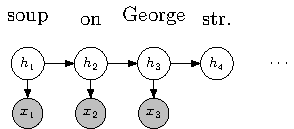
\includegraphics[width=0.5\textwidth]{figures/simple-crf.pdf}
  \end{centering}
  \caption{A conditional random field \todo{(arun): make a CRF and show what happens when measurements are added.}}
  \label{fig:crf}
\end{figure}

Conventionally, we are given a training dataset $\sD = \{\bx_i, \by_i\}$ and can learn $\theta$ by optimizing the convex log-likelihood objective $\sL(\theta) = \sum_{t=1}^T \log \p(\by\oft{t} \given \bx\oft{t})$.
In our setting, however, we do not observe the gold labels $\by$. 
Instead, we can ask the crowd to provide a ``measurement'' for some subset of the labels.
Let $\Sigma = \{\sigma_i\}$ be the set of possible measurements we can ask the crowd for and 
let $\by_\sigma \subseteq \by$ be the subset of labels queried.
The responses, $\tau_\sigma$, are modeled with an exponential measurement model as in~\cite{liang09measurements}:
\begin{align*}
  p(\tau_\sigma \given x, y) 
  &\propto \exp \left( \theta'^\top\phi'(\tau_\sigma, \bx, \by_\sigma) \right),
\end{align*}
where $\theta'$ and $\phi'$ are extra parameters and features.
The choice of an exponential model allows us to simply include measurements as an additional factor.

\paragraph{Running example}
As a running example, consider the conditional random field in \figureref{crf}. \todo{(arun): More details}

In the simplest case, we assume the labeler returns the true label with a uniform probability of $1- \epsilon$, and guesses at random otherwise, $\theta'$ and $\phi'$ are:
\begin{align*}
  \theta' &= 
      \begin{bmatrix}
        1 - \e \\ \e
      \end{bmatrix} &
  \phi'(\tau_\sigma, \by_\sigma, \bx) &=
    \begin{bmatrix}
      \BI[\tau_\sigma = y_\sigma] \\
      \BI[\tau_\sigma \neq y_\sigma]
    \end{bmatrix}.
\end{align*}
We revisit the problem of learning the error distribution of labelers in \sectionref{modeling-workers}.

Now that we have a model for our labeling task and the measurements we
can get from it, let us study how we can (a) predict labels, (b) predict
confidence, (c) incorporate partial feedback.

\paragraph{Prediction}
Given parameters $\theta$, we can simply query our model for a maximum likelihood labeling:
$\byt \given \bx = \argmax_{\by} \p(\by \given \bx)$.
In general, this corresponds to a message passing in a factor graph.
If we ask for measurements $\sigma_1, \ldots, \sigma_n$ and receive measurement responses $\tau_1, \ldots, \tau_n$, we can simply ask for the ML estimate in the augmented model:
$\byt \given \bx, \tau_1, \ldots \tau_n = \argmax_{\by} \p(\by \given \bx, \tau_1, \ldots \tau_n)$.

\paragraph{Deciding what to measure}

Our goal is to choose our querying strategy to minimize an arbitrary loss function:
\[\sL(h_{\text{true}}, h, m, t)\]
$\sL$ takes as parameters the true state of the world $h_{\text{true}}$, our guess $h$, and the money $m$ and time $t$ spent arriving at our guess.
 By tweaking $\sL$ practitioners applying our framework can move to arbitrary points on the cost-delay-accuracy tradeoff surface.
 We deliberately make no assumptions about the form of $\sL$ while developing theory, and demonstrate several choices in our experiments.


Let $\ell(\by, \byt)$ be the loss incurred when if $\by$ is labeled $\byt$.
When presented with an example $\bx$ to label, our system estimates a loss of $\E_{p(\by \given \bx)}[\ell(\by, \byt)]$, where $\byt = \argmax_{\by} \p(\by \given \bx)$.
If we performed the measurement operator $\sigma$ and received a measurement $\tau$,
then our expected loss would be $\E_{p(\by \given \bx, \tau)}[\ell(\by, \byt(\tau))]$, where $\byt(\tau) = \argmax_{\by} p(\by \given \bx, \tau)$.
Intuitively, if we had perfect feedback, observing $\tau$ would provide use more information, reducing our risk.
However, taking measurements has an associated cost, $C(\sigma)$, a function of time and money that the designer must choose.
There is also a possibility that the measurement does not return a value (because of a timeout).

Let the CDF be $F_\sigma(t)$.
We model the utility of a particular measurement operation, given a time window $t_0$ to be:
\begin{align*}
U(\sigma)
&= F_\sigma(t_0) 
  \E_{p(\tau \given x, \sigma)} \left[\E_{p(\by \given \bx, \tau)}[\ell(\by, \byt(\tau))] \right]
  + (1 - F_\sigma(t_0)) 
    \left[\E_{p(\by \given \bx)}[\ell(\by, \byt)] \right]
  + C(\sigma).
\end{align*}

Without loss of generality, assume that the null measurement is free: $C(\sigma_0) = 0$.
Intuitively, this ensures that we will only ever choose to measure something if the expected reduction in risk is more than the cost of executing the measurement.

Let the label $\by$ have $n$ components: $\by = (y_1, ..., y_n)$.
Further, let us assume that the loss function $\ell$ decomposes over labels: $\ell(\by, \byt) = \sum_{i=1}^n \ell(y_i, \yt_i)$. 
Under this assumption, the expected utility of a single measurement operator $\sigma$ can be efficiently computed with $2L$ inference calls\footnote{The marginal inference query in lines 6 and 7 of \algorithmref{expected-utility} can be shared.} to the model using \algorithmref{expected-utility}.

The measurement operator to take is simply $\sigma^* = \argmin_{\sigma \in \Sigma} U(\sigma)$.

\begin{algorithm}
\renewcommand{\algorithmicrequire}{\textbf{Input:}}
\renewcommand{\algorithmicensure}{\textbf{Output:}}
  \caption{Computing expected utility $U(\sigma)$}
  \label{algo:expected-utility}
  \begin{algorithmic}[1]
    \REQUIRE Measurement operator $\sigma$, input $\bx$, models $p_\theta(\by \given \bx)$ and $p_\theta(\by \given \bx, \tau, \sigma)$, $F_\sigma$ and $t_0$.
    \ENSURE Expected utility $U(\sigma)$
    \STATE Let $y_\sigma$ be label(s) measured by operator $\sigma$.
    \STATE Compute $p_\theta(y_\sigma \given \bx)$ using marginal inference.
    \STATE Set $p_\theta(\tau \given \bx) \gets p_\theta(\tau \given y_\sigma, \bx) p_\theta(y_\sigma \given \bx)$.
    \STATE Initialize $u \gets (0, \dots, 0)$.
    \FORALL{$i \in [L]$}
    \STATE Compute $\byt = \argmax_{\by} p_\theta(\by \given \bx, \tau = i, \sigma)$ using marginal inference.
    \STATE Compute $p(y_j) = p_\theta(\by_j \given \bx, \tau = i, \sigma)$ for $j \in [n]$ using marginal inference.
    \STATE Update $u[i] \gets \p(\tau = i \given \bx) \E_{p(y_j)}[\ell(y_j, \yt_j)]$.
    \ENDFOR
    \STATE Return the expected utility: $\frac{\sum_{i=1}^L u[i] p_\theta(\tau = i \given x)}{\sum_{i=1}^L p_\theta(\tau = i \given x)}$
  \end{algorithmic}
\end{algorithm}

From a practical perspective, we need to execute multiple queries. We consider this in \sectionref{async}.

\paragraph{Learning from responses}

Recall that we do not have gold labels for our data, but noisy measurements, leaving us with an unsupervised model.
We use the stepwise online EM algorithm \cite{liang09online}.
Note that unlike conventional unsupervised problems, there is high correlation between the labels we receive, which means we're likely to learn something not stupid.

